\documentclass[11pt, oneside]{article}
\usepackage[letterpaper, margin=2cm]{geometry}
\usepackage{AERE546}
\usepackage{xspace}
\newcommand{\xb}{\bar{x}}
\newcommand{\yb}{\bar{y}}

\begin{document}
\noindent \textbf{\Large{Caleb Logemann \\
AER E 546 Fluid Mechanics and Heat Transfer I \\
Homework 5
}}

%\lstinputlisting[language=MATLAB]{H01_23.m}
\begin{enumerate}
  \item % #1 Done
    Solve the Laplace equation
    \[
      \partial^2_x \psi + \partial^2_y \psi = 0
    \]
    in the domain $0 \le x, y \le 1$, with
    \begin{gather*}
      \psi = \sin[2]{3n\pi y} \text{ on } x = 0 \\
      \psi = \sin[2]{3n\pi x} \text{ on } y = 0 \\
      \psi = 0 \text{ on } x = 1  \\
      \psi = 0 \text{ on } y = 1.
    \end{gather*}
    Obtain numerical solutions with $n = 1$ and $n = 3$.

    Use Gauss-Seidel with SOR.
    Stop either when the modulus of the residual either has dropped by a factor
    of $10^{-4}$ or after 2500 iterations.
    \begin{itemize}
      \item Provide the algorithm part of your code.
      \item Provide contour plots of streamfunctions for each of $15 \times 15$
        and $151 \times 151$ grids for both $n$ values.
      \item For the $151 \times 151$ grid and $n = 1$, on a single graph, plot
        residual versus iteration for each of the relaxation parameters
        $\lambda = 1$, $\lambda = 0.5$, $\lambda = 1.5$, and $\lambda = 1.95$.
        Plot as $\log[10]{residual/residual_0}$ versus iteration number.
        Use the $L_2$ norm
        \[
          residual = \norm[L_2]{\Delta \Psi} = \sqrt{\sum{i = 1}{I}{\sum{j = 1}{J}{(\Delta \Psi_{ij}^2)/(I \times J)}}}
        \]
    \end{itemize}

    The following is my algorithm for Gauss-Seidel with SOR.
    \lstinputlisting[language=MATLAB]{sor.m}
    The following are the contour plots that for the different values of $n$ and
    $N$.
    \begin{center}
      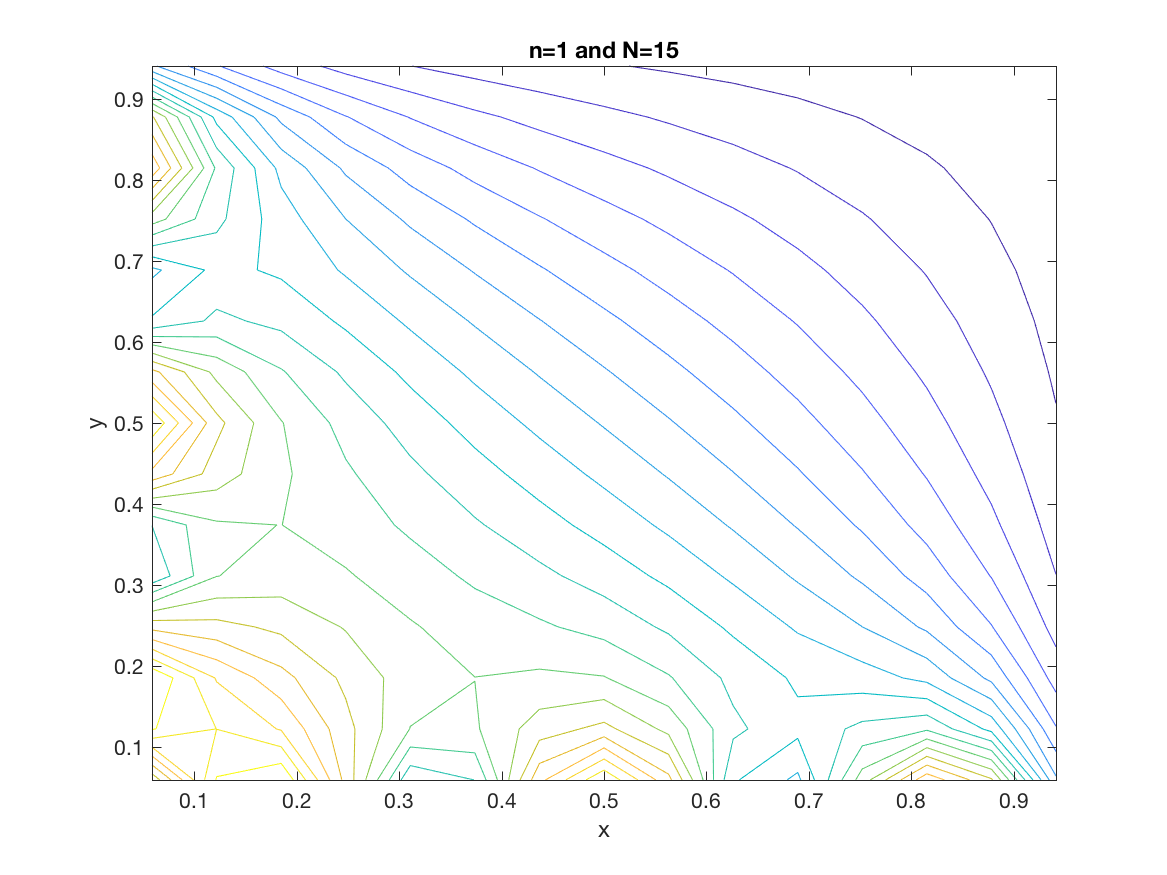
\includegraphics[scale=0.4]{Figures/05_1.png}
      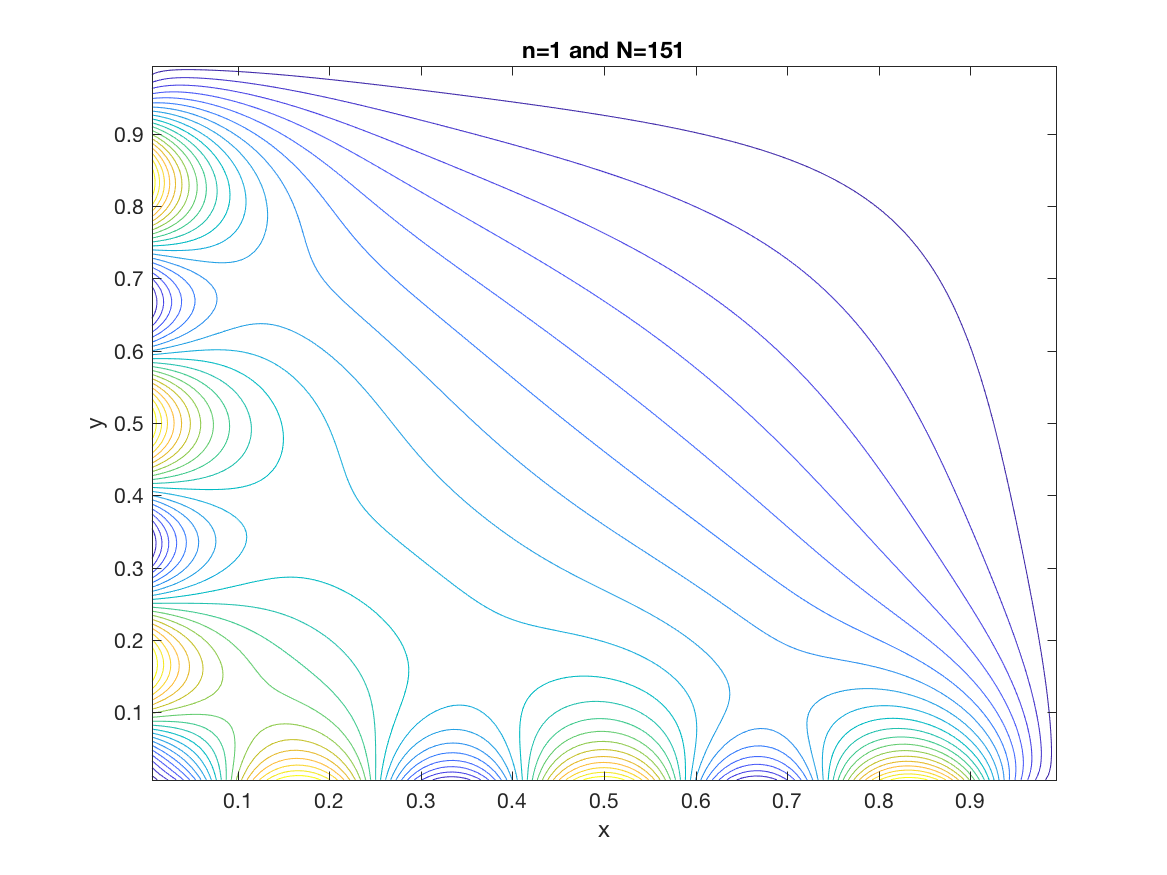
\includegraphics[scale=0.4]{Figures/05_2.png}
      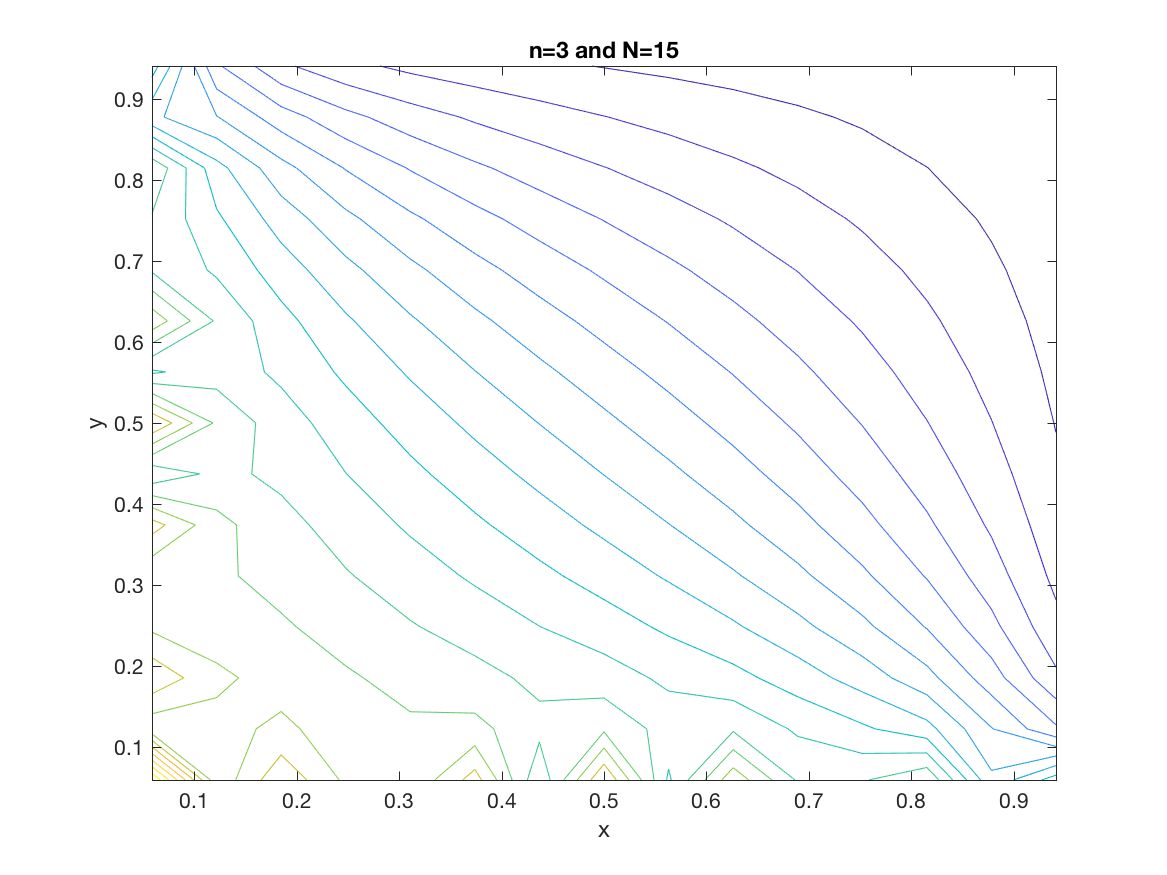
\includegraphics[scale=0.4]{Figures/05_3.png}
      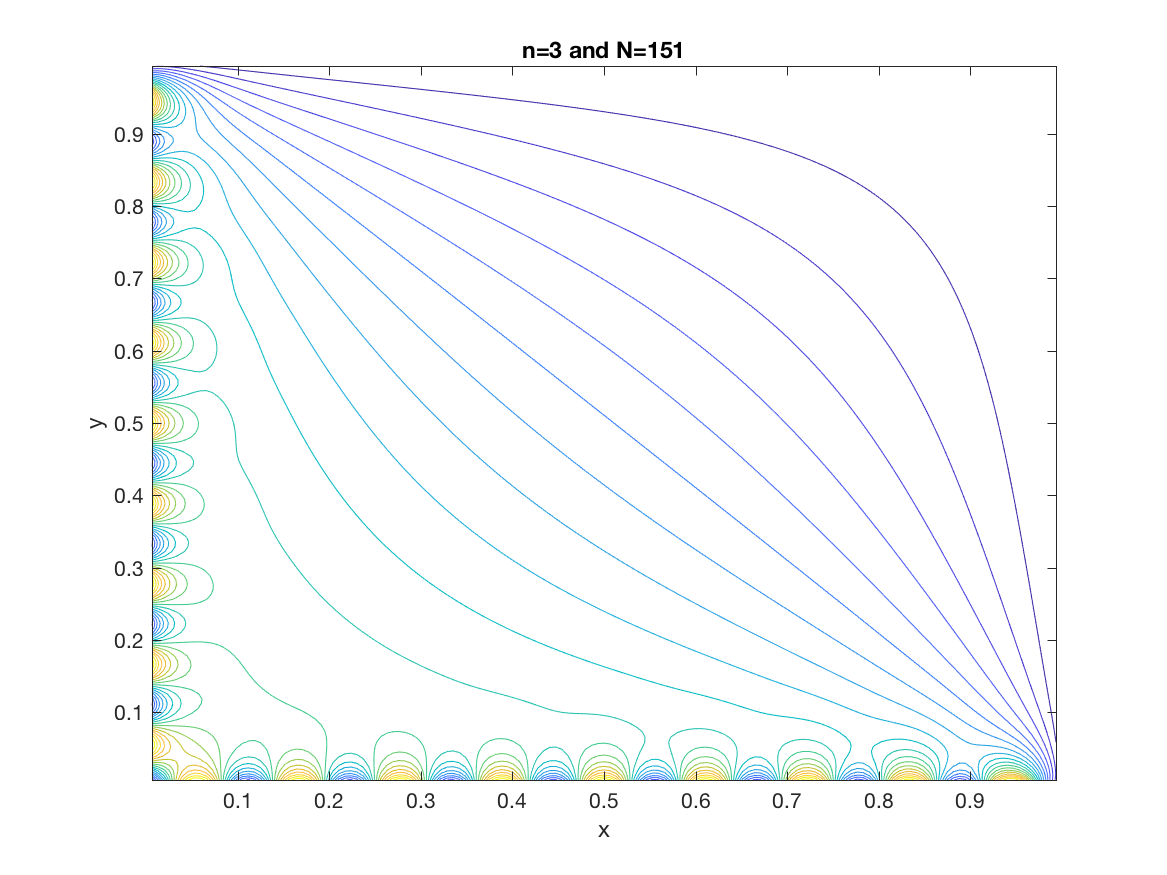
\includegraphics[scale=0.4]{Figures/05_4.png}
    \end{center}
    The following plot shows how the residual decreases with iteration for
    different values of $\lambda$.
    Note that only for $\lambda = 1.95$, did Gauss-Seidel with SOR converge
    within 2500 iterations.
    \begin{center}
      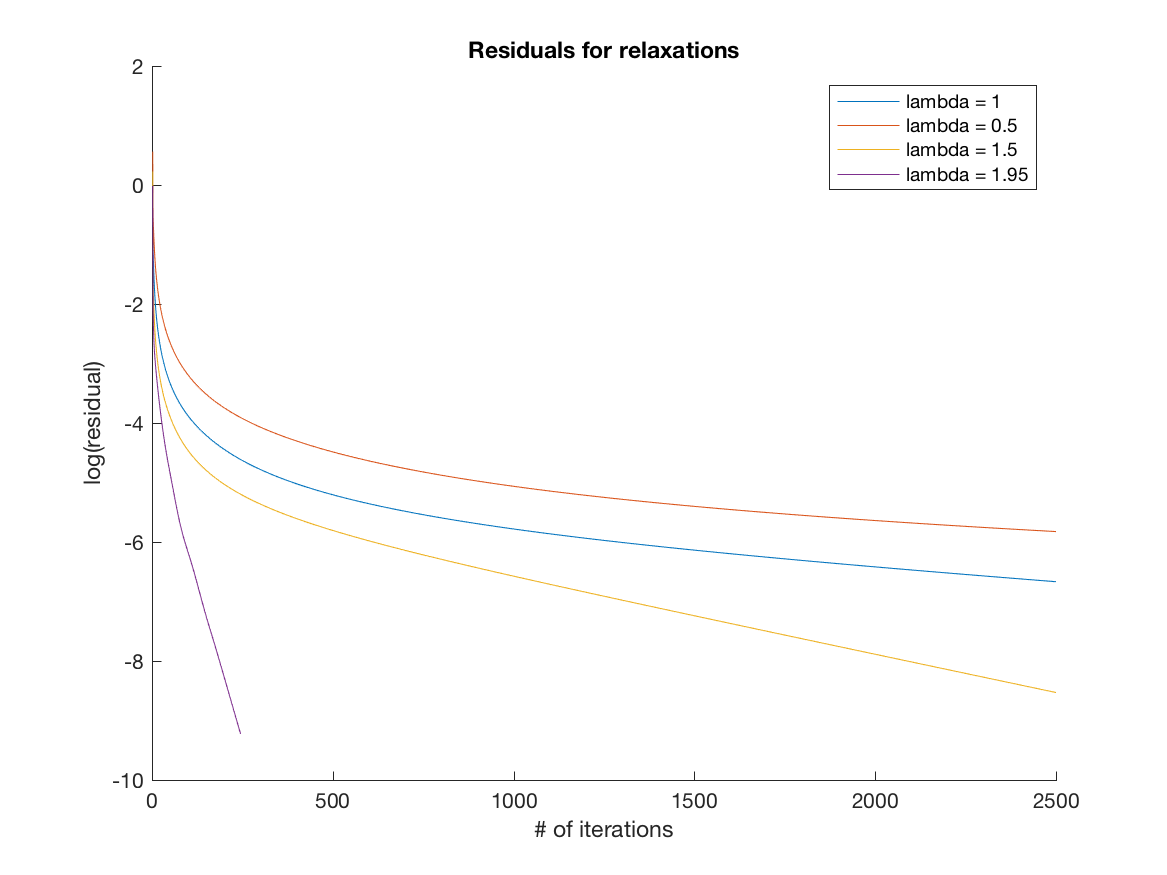
\includegraphics[scale=0.7]{Figures/05_5.png}
    \end{center}

  \item % #2 Done
    Solve the Poisson Equation
    \[
      \partial_x^2\psi + \partial^2_y\psi = 70e^{-32\p{(x - 0.5)^2 + (y - 0.1)^2}}
    \]
    in $0 \le x, y \le 1$, with boundary conditions
    \begin{gather*}
      \psi(0, y) = -y \\
      \psi(1, y) = -y \\
      \psi(x, 0) = 0 \\
      \psi(x, 1) = -1
    \end{gather*}
    on the grid
    \begin{gather*}
      x(j) = \frac{e^{2(j-1)/(J-1)} - 1}{e^2 - 1} \quad 1 \le j \le J \\
      y(j) = \frac{e^{2(k-1)/(K-1)} - 1}{e^2 - 1} \quad 1 \le k \le K.
    \end{gather*}
    \begin{itemize}
      \item Provide the algorithm part of your code.
      \item Provide a plot of the grid and a line-contour plot of the converged solution.
    \end{itemize}

    In order to solve this equation on this new grid we must do a change of
    variables.
    Since the new variables $\xb$ and $\yb$ depend only on $x$ and $y$
    respectively, a new equation can be created on a uniform grid,
    \[
      \pd[2]{\xb}{x} \pd{u}{\xb} + \p{\pd{\xb}{x}}^2 \pd[2]{u}{\xb}
      + \pd[2]{\yb}{y} \pd{u}{\yb} + \p{\pd{\yb}{y}}^2 \pd[2]{u}{\yb}
      = 70e^{-32\p{(\frac{e^{2\xb} - 1}{e^2 - 1} - 0.5)^2 + (\frac{e^{2\yb} - 1}{e^2 - 1} - 0.1)^2}}
    \]
    where
    \begin{align*}
      y &= \frac{e^{2\yb} - 1}{e^2 - 1} \\
      x &= \frac{e^{2\xb} - 1}{e^2 - 1}.
    \end{align*}
    Simplifying this equation gives
    \begin{align*}
      e^{-4\xb} \p{\pd{u}{\xb} - \frac{1}{2} \pd[2]{u}{\xb}} + e^{-4\yb} \p{\pd{u}{\yb} - \frac{1}{2} \pd[2]{u}{\yb}}
      = \frac{-140}{\p{e^2 - 1}^2} e^{-32\p{\p{\frac{e^{2\xb} - 1}{e^2 - 1} - 0.5}^2 + \p{\frac{e^{2\yb} - 1}{e^2 - 1} - 0.1}^2}}
    \end{align*}

    The following functions solve this modified equation.
    \lstinputlisting[language=MATLAB]{multByA2.m}
    \lstinputlisting[language=MATLAB]{solvePoisson.m}
    The following two images show the grid and the contour plot of the solution.
    \begin{center}
      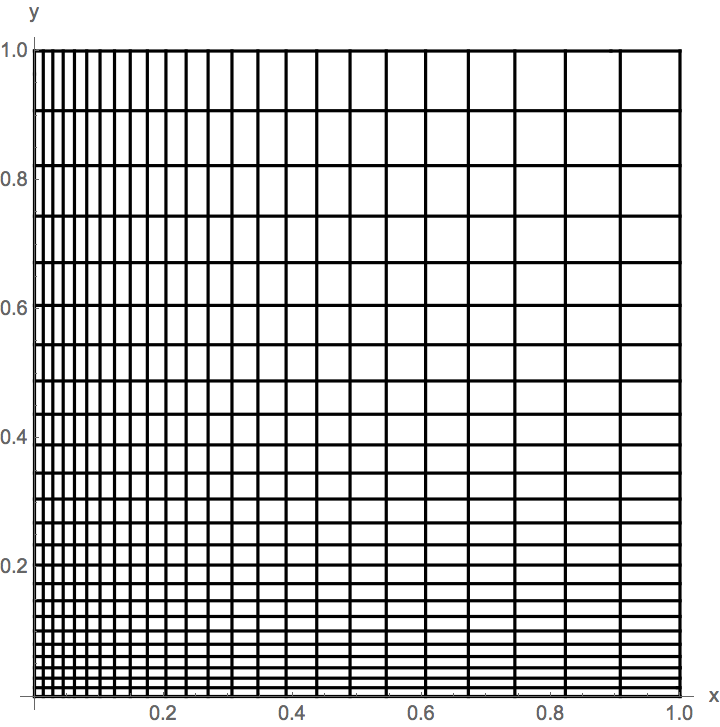
\includegraphics[scale=0.3]{Figures/05_06.png}
      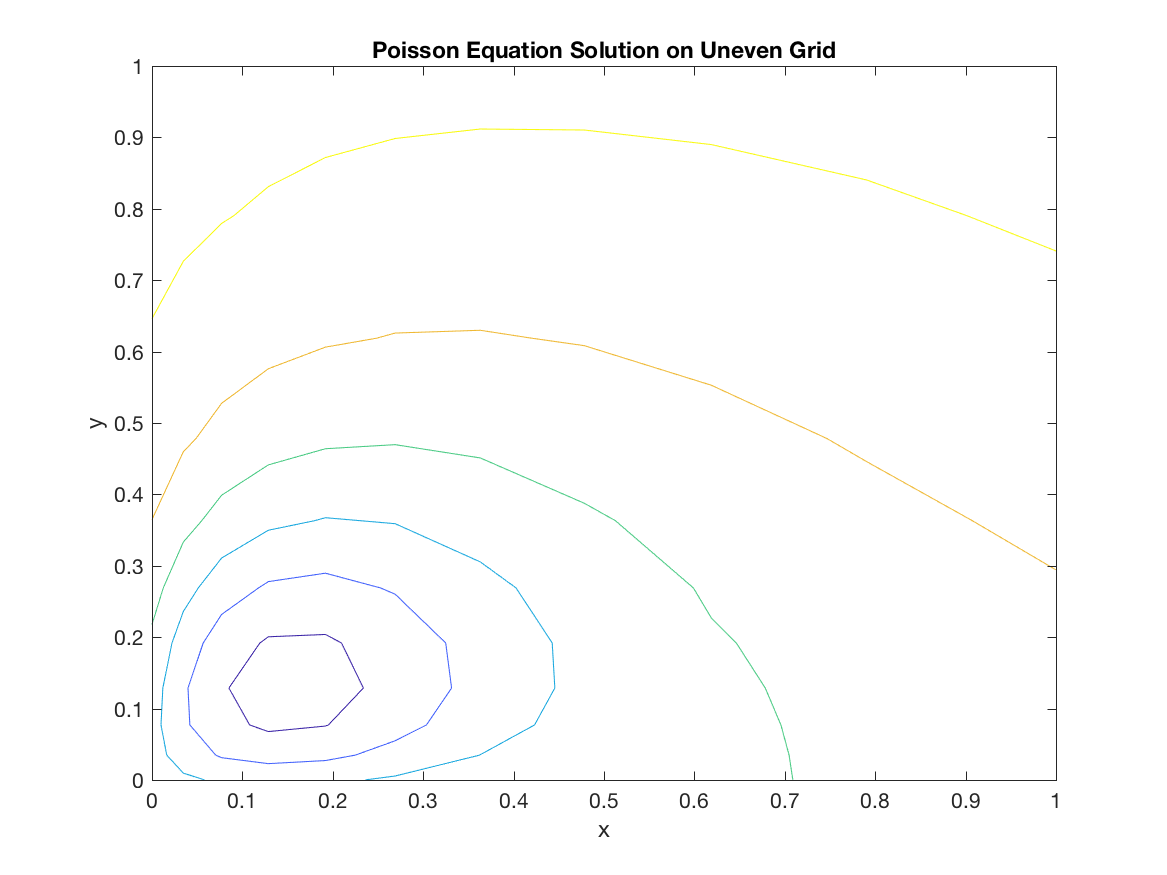
\includegraphics[scale=0.5]{Figures/05_07.png}
    \end{center}

  \item % #3 Done
    Solve the Poisson equation
    \[
      \partial^2_x \psi + \partial^2_y \psi = 2000\p{\sin{4 \pi x} \sin{4 \pi y}}^5
    \]
    on the domain $0 \le x \le 1$, $0 \le y \le 1$, with boundary conditions
    \begin{align*}
      \psi(x, 0) &= \sin[2]{\pi x} + 5\sin[2]{4\pi x} + 10 \sin[2]{8 \pi x} \\
      \psi(0, y) &= \sin[2]{4\pi y} \\
      \psi(x, 1) &= 0 \\
      \psi(1, y) &= 0
    \end{align*}
    Use a $151 \times 151$ grid.
    Submit only the algorithm part of your code.
    Plot $\log[10]{}$ of the residual - defined at
    $\norm[L_2]{\Delta \psi}/\norm[L^2]{\Delta \psi(0)}$ - versus iteration.
    Stop when the residual goes below $10^{-5}$.
    Provide a contour plot of the converged solution.

    The following is my conjugate gradient algorithm.
    \lstinputlisting[language=MATLAB]{conjugateGradient.m}
    The following images show a contour plot of the converged solution and a
    plot of the residual.
    The residual decreases as fast as Gauss-Seidel with SOR with weight $\lambda = 1.95$.
    \begin{center}
      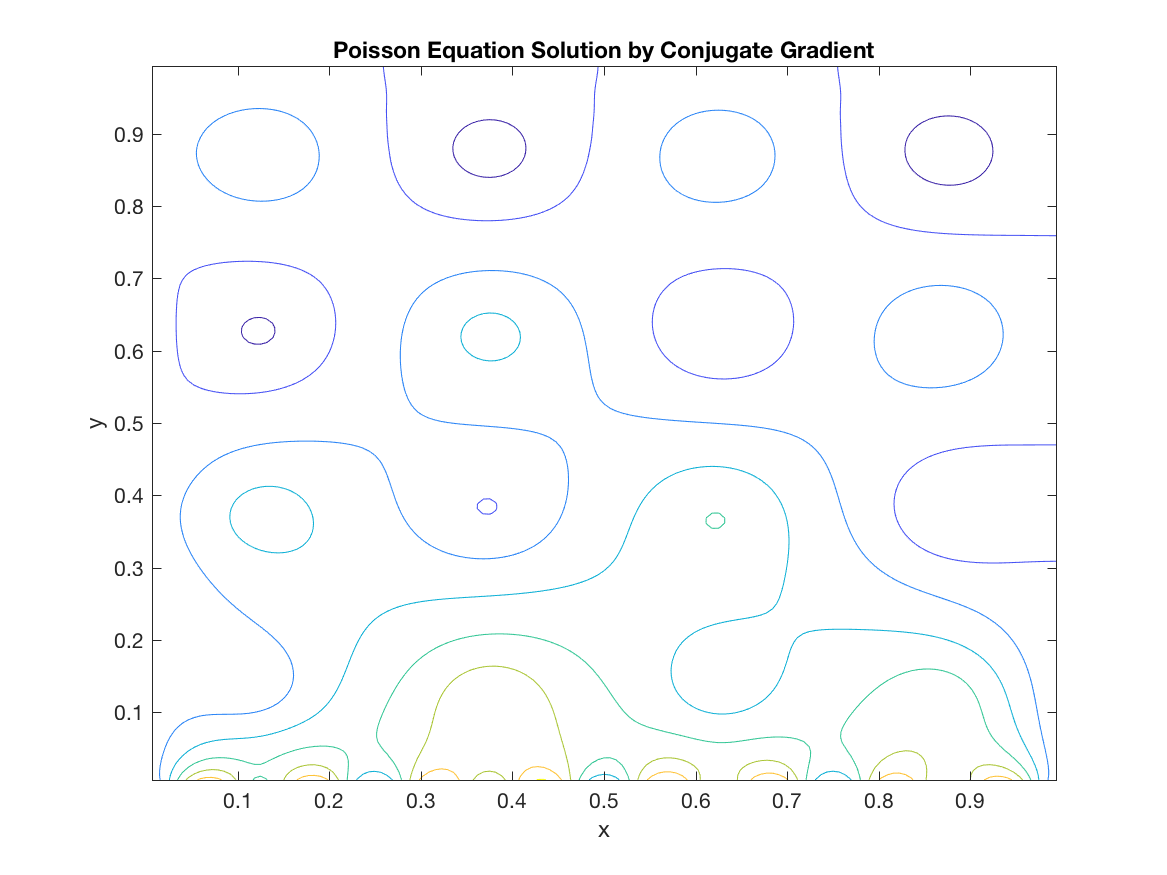
\includegraphics[scale=0.5]{Figures/05_8.png}
      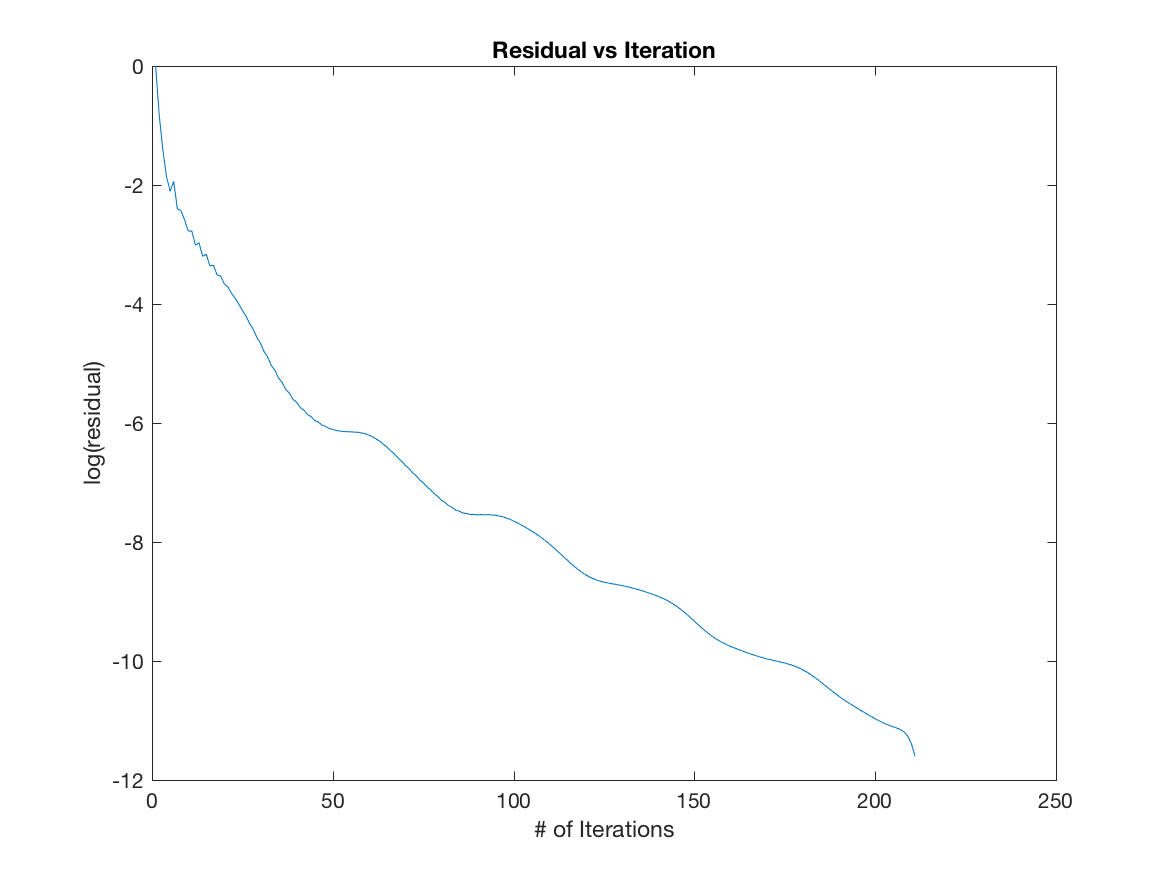
\includegraphics[scale=0.5]{Figures/05_9.png}
    \end{center}

\end{enumerate}
\end{document}
